\chapter{Fundamentação Teórica}
\label{cap2}

\section{Computação Paralela}

Há muito tempo o mercado de tecnologia vem buscando cada vez mais velocidade de processamento. Várias áreas demandam muito poder computacional para executar suas tarefas, desde o sequenciamento de DNA até simulações do universo, e para isso necessitam cada vez mais de um maior desempenho.

Antigamente, o aumento de desempenho estava diretamente atrelado ao aumento da frequência dos processadores. Porém, este aumento atingiu um limite físico para a velocidade do relógio. Quando mais rápida a frequência de relógio, menor deve ser o processador, pois os sinais elétricos devem ir e voltar dentro do mesmo ciclo de relógio. A solução para isso poderia ser a construção de uma \cpu cada vez menor, porém isso causa problemas de aquecimento, afinal uma maior frequência de relógio gera mais calor. Com a redução do tamanho da \cpu torna-se mais complicada a dissipação de calor da mesma.

Executar várias tarefas em paralelo, com várias \cpus trabalhando em conjunto, acabou sendo a forma encontrada para aumentar o poder computacional das máquinas. Hoje em dia já é possível encontrar arquiteturas paralelas com milhares de \cpus. Essas arquiteturas podem ser classificadas em dois grandes grupos: multiprocessadores e multicomputadores. No primeiro grupo (multiprocessadores) encontram-se as arquiteturas compostas por diversas \cpus interligadas através de um barramento ou similar, permitindo assim um compartilhamento da memória principal entre todas as \cpus. Por outro lado, no segundo grupo (multicomputadores), a memória principal é distribuída. A programação paralela nessas arquiteturas é feita através do uso de linguagens de programação, como o Erlang, e \apis, como o \mpi, desenvolvidos especialmente para computação paralela \cite{Tanenbaum2015}.

\subsection{Arquiteturas Paralelas}

Arquiteturas paralelas podem ser classificadas segundo seu fluxo de instruções e fluxo de dados utilizando a Taxonomia de Flynn\cite{Flynn1972}. A Tabela~\ref{tab:flynn} mostra as quatro classes possíveis de arquiteturas segundo esta classificação.

\begin{table}[t]
\centering
    \begin{tabular}{| l | p{6cm} | p{6cm} |}
    \hline
        & Único & Múltiplo \\ \hline
        Único & \sisd & \simd \\ \hline
        Múltiplo & \misd & \mimd \\ \hline
    \end{tabular}
    \caption{Taxonomia de Flynn}\label{tab:flynn}
\end{table}

\textbf{\sisd:} Um único fluxo de instruções trabalha em um único fluxo de dados. É a representação clássica de uma arquitetura sequencial. A Figura~\ref{fig:sisd} ilustra essa classe.

\begin{figure}[t]
    \centering
    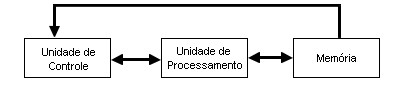
\includegraphics{Images/SISD.jpg}
    \caption{Classe SISD da Taxonomia de Flynn}\label{fig:sisd}
\end{figure}

\textbf{\simd:} Uma única instrução é responsável pelo processamento de vários dados. Define o funcionamento de processadores vetoriais e matriciais. Diversos módulos de memória são necessários, as instruções seguem organizadas sequencialmente e possui uma unidade de controle e várias unidades de processamento. A Figura~\ref{fig:simd} ilustra essa classe.

\begin{figure}[t]
    \centering
    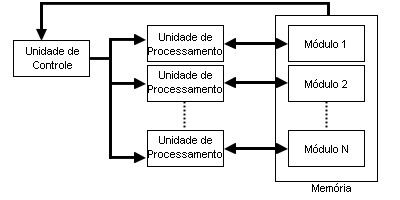
\includegraphics{Images/SIMD.jpg}
    \caption{Classe SIMD da Taxonomia de Flynn}\label{fig:simd}
\end{figure}

\textbf{\misd:} Múltiplas instruções trabalhando no mesmo fluxo de dados. Esta classe da Taxonomia de Flynn é impossível de ser colocada em prática. A Figura~\ref{fig:misd} ilustra essa classe.

\begin{figure}[t]
    \centering
    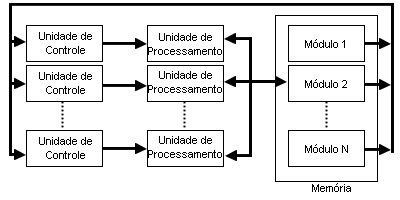
\includegraphics{Images/MISD.jpg}
    \caption{Classe MISD da Taxonomia de Flynn}\label{fig:misd}
\end{figure}

\textbf{\mimd:} Múltiplas instruções trabalhando em múltiplos dados. Possui várias unidades de controle, várias unidades de processamento e vários módulos de memória. Qualquer grupo de máquinas operando em conjunto, com interação entre elas, pode ser classificado como \mimd. A Figura~\ref{fig:mimd} ilustra essa classe.

\begin{figure}[t]
    \centering
    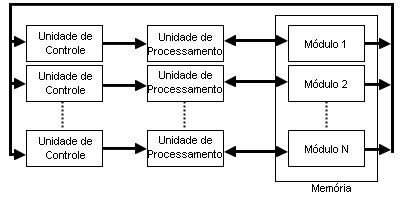
\includegraphics{Images/MIMD.jpg}
    \caption{Classe MIMD da Taxonomia de Flynn}\label{fig:mimd}
\end{figure}

Além da Taxonomia de Flynn, as arquiteturas paralelas podem ser classificadas segundo o compartilhamento de memória. Multiprocessadores trabalham com vários processadores podendo acessar a mesma memória compartilhada, enquanto nos multicomputadores cada processador possui sua própria memória, fazendo necessário o uso de uma rede de interconexão para trocar informações.

\subsubsection{Multiprocessadores}

Multiprocessadores são sistemas nos quais múltiplas \cpus compartilham acesso à mesma memória. Uma propriedade que forma a base da comunicação entre processadores é: uma \cpu escreve algum dado na memória e outra lê o mesmo dado. Sistemas multiprocessadores possuem algumas características únicas, como sincronização de processos e escalonamento, por exemplo. A Figura~\ref{fig:mproc} exibe graficamente a arquitetura de um multiprocessador.

\begin{figure}[t]
    \centering
    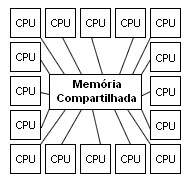
\includegraphics{Images/Multiprocessador.jpg}
    \caption{Multiprocessador}\label{fig:mproc}
\end{figure}

Alguns multiprocessadores possuem a característica de que uma certa palavra de memória possa ser lida na mesma velocidade que qualquer outra palavra. Essas máquinas são chamadas de \uma. Máquinas que não apresentam essa propriedade são chamadas de \numa \cite{Tanenbaum2015}.

\subsubsection{Multicomputadores}

Multicomputadores são sistemas nos quais cada \cpu possui sua própria memória, não podendo ser diretamente acessada por nenhum outro processador. A troca de informações nesse sistema é feita através de uma rede de interconexão. A Figura~\ref{fig:mcomp} exibe graficamente a arquitetura de um multicomputador.

\begin{figure}[t]
    \centering
    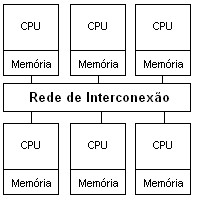
\includegraphics{Images/Multicomputador.jpg}
    \caption{Multicomputador}\label{fig:mcomp}
\end{figure}

O acesso à memória nos multicomputadores é classificado como \norma, afinal não é possível que uma \cpu tenha acesso à memória remota \cite{Hwang1998}.

\subsubsection{Aceleradores}

Uma \gpgpu, ou um acelerador, é uma placa gráfica que pode ser usada para computação de propósito geral. São classificados como \simd pela Taxonomia de Flynn, permitindo que vários dados possam ser processados em paralelo. As placas atuais utilizam uma extensão desse conceito, chamada de \simt, garantindo a execução da mesma instrução em threads diferentes. A Figura~\ref{fig:acel} exibe graficamente a arquitetura de um acelerador.

\begin{figure}[t]
    \centering
    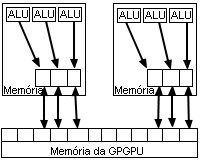
\includegraphics{Images/gpgpu.jpg}
    \caption{Acelerador}\label{fig:acel}
\end{figure}

\gpgpus são compostas por vários processadores, que possuem vários núcleos cada, sendo que cada processador possui sua própria memória interna, compartilhada pelas suas \alus, e uma memória compartilhada entre todos os processadores \cite{Miranda2010}.

\subsection{Programação Paralela}

As técnicas, linguagens ou \apis para o desenvolvimento de aplicações paralelas estão, em grande parte dos casos, diretamente atreladas às arquiteturas. Por exemplo, para multicomputadores o modelo de programação mais difundido para paralelismo é o \mpi. No caso de \gpus e aceleradores o \cuda e o \opencl são os mais utilizados.

Neste trabalho, iremos focar em arquiteturas de memória compartilhada (multiprocessadores). Para este tipo de arquitetura, uma das \apis mais aceitas e utilizadas é o \openMP.

O \openMP é baseado em diretivas de compilação, podendo ser usado em C/C++ ou em Fortran, combinando regiões sequenciais e paralelas no mesmo código fonte. As diretivas permitem a criação de regiões paralelas nas quais múltiplas threads são criadas e executadas em paralelo. O número de threads em uma região paralela pode ser determinado pelo usuário, todavia, em programas paralelos utiliza-se normalmente uma thread para cada núcleo de processamento da arquitetura \cite{Chapman2008}.

Para C/C++ as diretivas são da seguinte maneira:
\begin{center}
\texttt{\#pragma omp [diretiva] [atributos]}
\end{center}

Variáveis globais são compartilhadas entre as threads, porém variáveis criadas dentro de um laço são privadas. Para uma variável declarada fora do laço ter um contexto privado para cada thread, é necessário o uso do atributo \texttt{private}, da seguinte forma:
\begin{lstlisting}
    int i, j;
    
    #pragma omp parallel for private(j)
    for (i = 0; i < 10; i++) {
        for (j = 0; j < 10; j++) {
            ...
        }
    }
\end{lstlisting}

Quando existem dois ou mais laços aninhados, é possível utilizar o atributo \texttt{collapse}. Este atributo unifica os laços em um único e grande laço, o qual será dividido entre as threads. A diretiva \texttt{collapse} recebe como parâmetro a quantidade de laços para serem unificados, da seguinte forma:
\begin{lstlisting}
    #pragma omp parallel for collapse(2)
    for (int i = 0; i < 10; i++) {
        for (int j = 0; j < 10; j++) {
            ...
        }
    }
\end{lstlisting}

Existem algumas opções de escalonadores para serem utilizados pelo \openMP. Eles servem para definir como as threads dividirão as tarefas que serão executadas.

Os tipos de escalonadores são o \texttt{static}, escalonador padrão do \openMP que divide igualmente as tarefas entre as threads, o \texttt{dynamic}, escalonador que recebe um tamanho de bloco como parâmetro, divide as tarefas em blocos com este tamanho e as threads vão pegando o próximo bloco assim que ficam ociosas, e o \texttt{guided}, escalonador semelhante ao \texttt{dynamic}, porém os blocos são grandes no começo e vão diminuindo exponencialmente \cite{Chandra2000}.

A diretiva que define o escalonador funciona da seguinte forma:
\begin{lstlisting}
    #pragma omp parallel for schedule(ESCALONADOR, TAMANHO DO BLOCO)
    for (int i = 0; i < 10; i++) {
        ...
    }
\end{lstlisting}

Quando existem vários laços independentes dentro de uma mesma região paralela, é possível utilizar a diretiva \texttt{nowait} para evitar que uma thread ociosa precise esperar um laço acabar para poder executar o próximo laço.
É usada da seguinte maneira:
\begin{lstlisting}
    #pragma omp parallel
    for (int i = 0; i < 10; i++) {
        #pragma omp for nowait
        for (int j = 0; j < 10; j++) {
            ...
        }
        
        #pragma omp for nowait
        for (int j = 0; j < 10; j++) {
            ...
        }
    }
\end{lstlisting}

A Figura~~\ref{fig:lstopenmp} exemplifica o uso do \openMP na soma de duas matrizes. É usada a diretiva \texttt{parallel} para iniciar uma região paralela, \texttt{for} para paralelizar o laço entre as threads, \texttt{schedule} para definir o escalonamento como \texttt{guided} e \texttt{private} para definir a variável \texttt{j} como privada para cada thread. 

\begin{figure}[t]
    \centering
    \begin{lstlisting}
    int i, j;
    
    #pragma omp parallel for schedule(guided) private(j)
    for (i = 0; i < 1000; i++) {
        for (j = 0; i < 1000; j++) {
            a[i][j] = b[i][j] + c[i][j];
        }
    }
    \end{lstlisting}
    \caption{Soma de matrizes usando OpenMP.}
    \label{fig:lstopenmp}
\end{figure}

O sucesso do \openMP se deve ao fato de que ele é bem simples de ser usado e, por conta de uma alta aceitação, consegue ser executado em várias plataformas diferentes \cite{Chapman2008}.

\section{Criptografia de Dados}

Do grego \textit{Kriptos} (oculto) e \textit{Grapho} (escrita), é o nome dado à ciência de codificar e decodificar mensagens. Tem como meta garantir:
\begin{itemize}
    \item \textbf{Autenticação}: Identificar o remetente da mensagem;
    \item \textbf{Integridade}: Não adulteração da mensagem original;
    \item \textbf{Não Recusa}: Remetente não pode negar que enviou a mensagem.
\end{itemize}

A criptografia pode ser classificada como simétrica ou assimétrica, dependendo de como as chaves de codificação e decodificação são utilizadas. Há também o resumo criptográfico, ou Hash, que é um número pequeno que representa todo um documento \cite{Stallings2014}.

\subsection{Criptografia Simétrica}

O conceito mais antigo de criptografia é chamado de criptografia simétrica. Neste modelo a chave que dá acesso à mensagem é a mesma, tanto para codificar como para decodificar a mensagem, e deve permanecer em segredo, por isso é chamada de chave privada. A chave é utilizada para evitar que terceiros tenham acesso à mensagem, mesmo conhecendo o algoritmo utilizado e tendo em mãos a mensagem cifrada. A Figura~\ref{fig:cripsim} exibe o funcionamento da criptografia simétrica.

A maior vantagem da criptografia simétrica é sua facilidade de uso e velocidade para executar os algoritmos criptográficos. O problema deste modelo é que a chave usada para cifrar precisa ser compartilhada com o destinatário, abrindo uma brecha para terceiros interceptarem a chave \cite{Stallings2014}.

\begin{figure}[t]
    \centering
    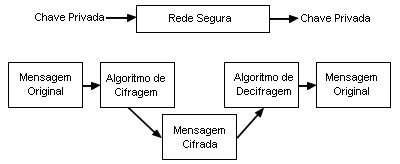
\includegraphics{Images/Simetrica.jpg}
    \caption{Criptografia Simétrica}\label{fig:cripsim}
\end{figure}

Os principais algoritmos de criptografia simétrica são:
\begin{itemize}
    \item \aes: Desenvolvido pelo \textit{National Institute of Standards and Technology}, é o algoritmo padrão usado pelo governo dos Estados Unidos da América. Possui um tamanho de bloco fixo em 128 bits, chave de 128, 192 ou 256 bits, rápido e fácil de executar e utiliza pouca memória.
    \item \des: Desenvolvido pela IBM em 1977, foi o algoritmo mais utilizado no mundo até a padronização do \aes. Possui um tamanho de chave pequeno, de apenas 56 bits, o que possibilita quebrar o algoritmo por força bruta. A partir de 1993 passou a ser recomendada a utilização do 3DES, uma variação do \des no qual o ciframento é feito 3 vezes seguidas, porém é muito lento para se tornar um algoritmo padrão.
\end{itemize}

\subsection{Criptografia Assimétrica}

Modelo desenvolvido pelo matemático Clifford Cocks, no qual as chaves para cifrar e decifrar são diferentes, chamadas de assimétricas. A chave pública pode ser vista por qualquer pessoa, porém a chave privada permanece em posse apenas do titular. Uma pessoa pode utilizar sua chave privada para decodificar uma mensagem criptografada com sua chave pública. A Figura~\ref{fig:cripasim} exibe o funcionamento da criptografia assimétrica.

A maior vantagem deste modelo é a segurança, uma vez que a chave privada não é compartilhada. Porém a velocidade é muito menor do que os algoritmos simétricos, o que pode não permitir o seu uso em algumas situações \cite{Stallings2014}.

\begin{figure}[t]
    \centering
    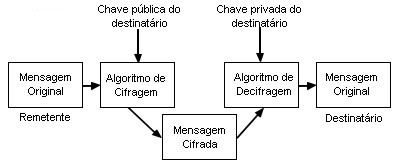
\includegraphics{Images/Assimetrica.jpg}
    \caption{Criptografia Assimétrica}\label{fig:cripasim}
\end{figure}

Os principais algoritmos de criptografia assimétrica são:
\begin{itemize}
    \item \rsa: Desenvolvido em 1977 no \mitt. É o algoritmo assimétrico mais utilizado no momento, além de ser um dos mais poderosos que existem. É baseado no fato de que dois números primos são facilmente multiplicados para gerar um terceiro número, porém é muito difícil recuperar esses números a partir do terceiro número. Para se descobrir a chave privada, é necessário fatorar números muito grandes, o que pode levar um tempo considerável. Assim, a segurança do RSA é baseada na dificuldade de fatoração de números primos grandes.
    \item \elgamal: Baseado em grandes cálculos matemáticos. Sua segurança é baseada na dificuldade de calcular logaritmos discretos em um corpo finito.
    \item \dhes: Mais antigo dos métodos assimétricos, também é baseado no problema dos logaritmos discretos. Não é possível usá-lo para assinaturas digitais.
\end{itemize}

\subsection{Resumo Criptográfico}

Resumo criptográfico, também conhecido por hash, são funções criptográficas unidirecionais, ou seja, não é possível obter o conteúdo original a partir do hash. Uma característica dessas funções é que, independente do tamanho do texto, hash sempre terá um tamanho fixo, geralmente de 128 bits. Outra propriedade é que duas mensagens distintas não irão gerar o mesmo hash \cite{Pfleeger2015}.

Os principais algoritmos de hash utilizados atualmente são:
\begin{itemize}
    \item \mdd: Desenvolvido por Ron Rivest, do \mitt. Produz um hash de 128 bits. É um algoritmo rápido, simples e seguro, porém não é recomendado devido ao pequeno tamanho de 128 bits, sendo preferível um hash de maior valor.
    \item \sha: Criado pela \nsa, gera um hash de 160 bits. É recomendável o uso do \sha-2, uma variação mais forte e segura do que o \sha-1, devido ao maior número de bits que é gerado.
\end{itemize}

Alguns usos de funções de hash são:

\begin{itemize}
    \item \textbf{Verificar integridade de arquivos}: Basta tirar o hash de um arquivo e guardá-lo. Em um momento futuro é possível tirar o hash novamente e comparar com o antigo, se forem iguais então o arquivo está íntegro.
    \item \textbf{Armazenamento de senhas}: A forma mais segura de armazenar uma senha é armazenar o hash da mesma, afinal não é possível obter a senha original. Quando precisar ser feita a verificação se uma senha digitada está correta, basta comparar o hash da senha digitada com o hash armazenado, se forem iguais então a senha está correta.
\end{itemize}

\section{Compressão de Dados}

Comprimir dados é o ato de reduzir o tamanho de arquivos, diminuindo o espaço que eles ocupam em disco e aumentando o desempenho de aplicativos que usam esses dados. Essa técnica é interessante para diversos fins, desde um usuário de smartphone que deseja armazenar mais fotos no seu aparelho até um serviço \textit{web} que envia muitos dados através da internet. A Figura~\ref{fig:compression} mostra o conceito da compressão de dados.

Existem duas formas de compressão, com perdas e sem perdas, que descartam partes insignificantes do arquivo ou mantém todo o conteúdo, respectivamente.

\begin{figure}[t]
    \centering
    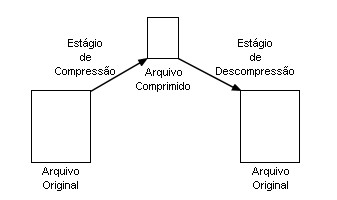
\includegraphics{Images/Compressao.jpg}
    \caption{Compressão de Dados}\label{fig:compression}
\end{figure}

\subsection{Compressão sem Perdas}

A compressão sem perdas, ou \textit{Lossless Data Compression}, garante que os dados obtidos após a descompressão serão exatamente iguais aos dados originais que foram comprimidos. Essa técnica é geralmente utilizada quando não se pode perder nada do conteúdo original, como arquivos de texto ou informações delicadas de experimentos científicos por exemplo.

\subsection{Compressão com Perdas}

A compressão com perdas, ou \textit{Lossy Data Compression}, garante que os dados obtidos após a descompressão serão bastante parecidos com o conteúdo original, com diferenças mínimas. Essa técnica é geralmente utilizada para arquivos de áudio ou vídeo, nos quais a diferença de conteúdo é imperceptível e o tamanho é reduzido consideravelmente.

\subsection{Compressão de Textos}

A compressão de textos se baseia em representar o texto original de outra maneira, usando símbolos que ocupem menos espaço. Com isso se ganha também velocidade ao se fazer busca em grandes documentos. A desvantagem é o tempo necessário para a descompressão do conteúdo.

Um dos métodos mais conhecidos é o método de Huffman, de 1952. Nele, um código único é associado a cada caractere diferente do texto. Códigos menores são associados com os caracteres que aparecem com maior frequência. É o método mais eficiente para compressão de textos em linguagem natural, com 60\% de redução no tamanho do arquivo. O método de Huffman elimina todos os espaços entre palavras. No momento da descompressão, a não ser que exista um separador, como uma vírgula, um espaço é inserido entre as palavras \cite{Salomon2007}.

\subsection{Compressão de Imagens}

Existem formatos de imagens que comprimem com ou sem perdas. Os mais conhecidos formatos de compressão sem perdas são \png, \jpegg e \tiff.

A compressão sem perdas explora a redundância entre pixeis e garante que nenhum dado será perdido. É especialmente importante em casos nos quais a fidelidade dos dados é muito importante, como para a fotografia profissional. Os algoritmos mais usados são o \rle, \lz, \lzw e o algoritmo de Huffman, o qual é usado nos formatos \png e \tiff.


Dentre os métodos com perdas, os mais conhecidos são \jpeg e \gif. A compressão com perdas busca eliminar detalhes que não são perceptíveis ao olho humano. Porém há formatos, como o \gif, que utilizam um grau maior de perda, causando uma degradação grande na imagem.

%\subsubsection{A Transformada DCT}
%
%A transformada discreta do cosseno é similar à transformada de Fourier, porém utiliza apenas números reais. É esperado que os pixeis de uma imagem tenham uma transição contínua de um para outro. A \dct consiste em encontrar uma base na qual os primeiros elementos terão pouca variação, e os últimos terão grande variação. Assim, podemos escrever os pixeis da imagem como uma combinação linear da base, na qual os últimos coeficientes são praticamente nulos, podendo ser eliminados.
%
%Como uma imagem é representada como uma matriz de pixeis, é utilizada a \dct bidimensional, no qual a transformada é aplicada primeiramente nas linhas e depois nas colunas. A equação da transformada para uma imagem \textit{P} de tamanho \textit{n X n} é dada pela seguinte equação \cite{ahmed1974}:
%
%\begin{equation}
%    Gij=\frac{1}{\sqrt{2n}}CiCj\sum_{x=0}^{n-1}\sum_{y=o}^{n-1} Pxy \;  \cos\bigg(\frac{(2y+1)j\pi}{2n}\bigg) \;  %\cos\bigg(\frac{(2x+1)i\pi}{2n}\bigg)
%\end{equation}
%para $$0 \leqslant i, j \leqslant n-1$$
%onde $$Cf=\frac{1}{\sqrt{2}}, f=0\quad ou \quad Cf=1,f>0$$
%
%A recuperação dos dados originais é feita através da transformação inversa, conhecida por \idct bidimensional:
%
%\begin{equation}
%    Pxy=\frac{1}{4}\sum_{i=0}^{n-1}\sum_{j=0}^{n-1}CiCjCij \;
%    \cos\bigg(\frac{(2x+1)i\pi}{2n}\bigg) \;
%    \cos\bigg(\frac{(2y+1)j\pi}{2n}\bigg)
%\end{equation}
%
%\todo[inline]{Aqui vale um comentário. A fórmula é bonita, mas sabes explicá-la? Simplesmente colocar uma fórmula no texto e não saber explicá-la não faz muito sentido. Nesse caso, aqui precisa ser adicionado um texto para explicar as duas equações apresentadas anteriormente.}